\begin{figure}[htbp]
\centering
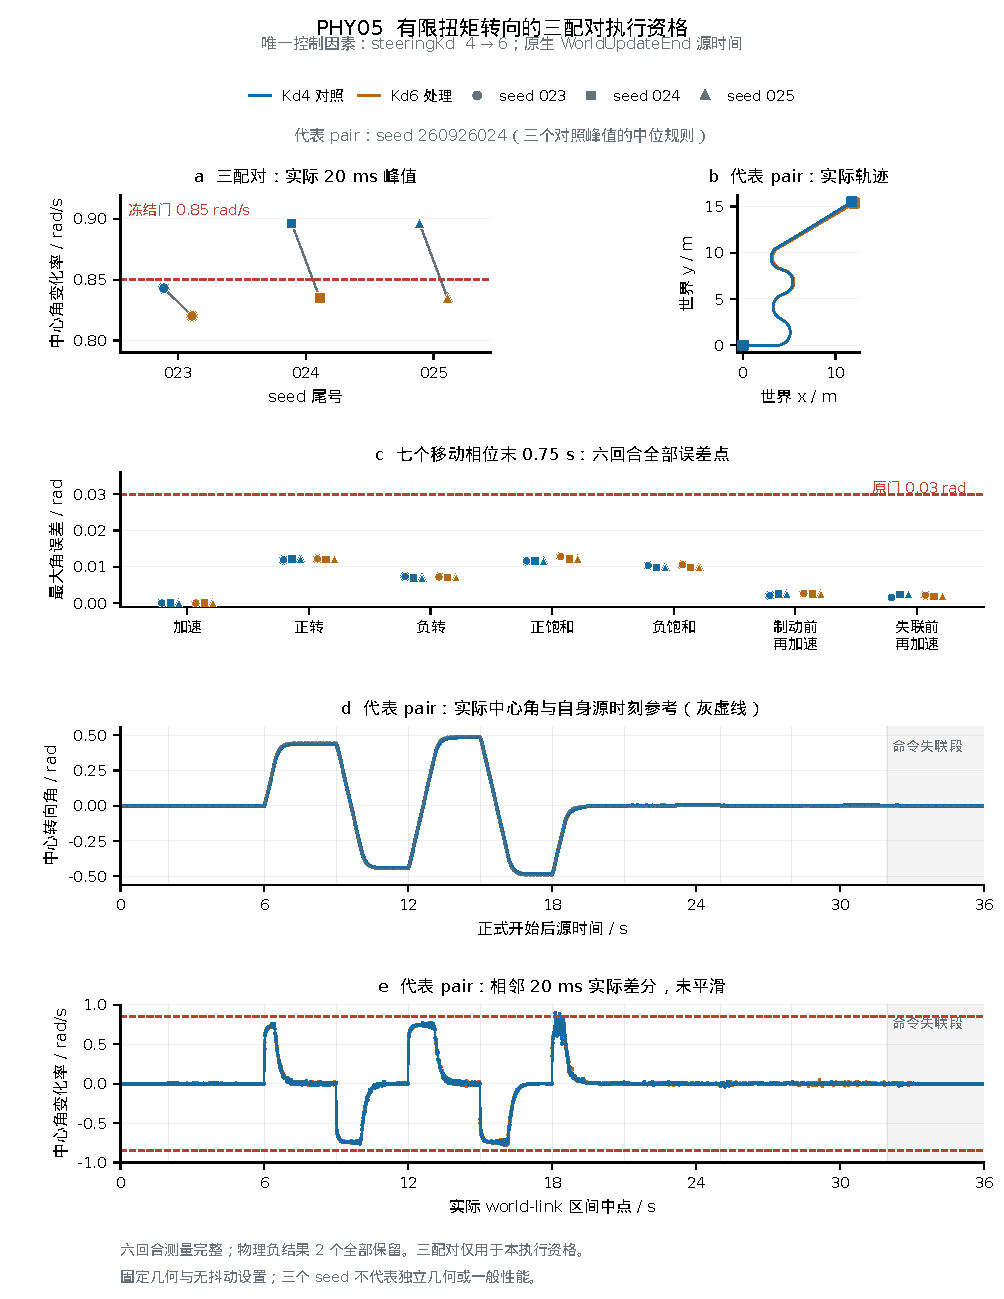
\includegraphics[width=170mm]{PHY05.pdf}
\caption{P07三配对有限扭矩执行资格，唯一控制因素为steeringKd4→6，六回合均保留。a展示三个fresh seed的原生20ms实际world-link中心转向斜率绝对峰值；对照/处理依次为260926023：0.843004/0.820135，260926024：0.896392/0.834795，260926025：0.896392/0.834795 rad/s，红虚线为冻结0.85rad/s门。b展示预注册规则选出的seed260926024实际世界轨迹：按三个control峰值升序（完全同值按seed）取中位，处理结果不参与选择。c为七个具有原稳定转向门的移动相位，每相位展示六回合全部点；误差来自固定末0.75s整数半开窗口内原生实际角的最大绝对偏差，红线为0.03rad原门，全部11相位数字另附CSV。d/e展示该代表pair完整36s、未平滑未重采样的实际中心角及20ms差分，参考角保留各自50Hz源时刻；曲线不移到joint/target相位。中心角由base\_link相对左右steer\_link四元数，经独立左右Ackermann曲率平均反演。六回合均通过source、bag、暂停watermark和ingress测量审计；2个原物理负结果完整保留，原失败检查为m12\_physics\_p07\_s024\_kd4: actual\_center\_slew\_with\_declared\_sampling\_tolerance; m12\_physics\_p07\_s025\_kd4: actual\_center\_slew\_with\_declared\_sampling\_tolerance。该图不将3个仿真seed配对外推为一般导航性能、物理安全或真实车结果；500Hz诊断不替代冻结20ms资格门。 补充采样尺度诊断：三个Kd6回合的原生2ms峰值依次为0.855811, 0.845847, 0.845847 rad/s；seed023的2ms峰仍超过0.85，故20ms资格通过不代表每physicsstep都满足同一界。固定几何和无噪声/无抖动条件下，seed024/025两臂20ms峰完全相同，三对不是独立几何或泛化统计。}
\label{fig:phy05-actuation-qualification}
\end{figure}
